\section{Bewegungsplanung}

\textbf{Ziel}: Erzeugen einer kollisionsfreien Trajektorie unter Berücksichtigung verschiedener Ziele und Einschränkungen

\textbf{Arbeits- und Konfigurationsraum}:
\begin{itemize}
	\item \textbf{Arbeitsraum} $W$: Kartesischer Raum $\R^6$, in dem sich der \textbf{Tool Center Point} (TCP) aufhalten kann
	\item \textbf{Konfiguration} $\mathbf{q}\in C$ beschreibt den Zustand eines Roboters als Gelenkwinkelvektor im Gelenkwinkelraum
	\item \textbf{Konfigurationsraum} $C=C_\text{free}\cup C_\text{obs}\,$: $n$-dimensionaler Raum aller Gelenkwinkelkonfigurationen
	\item \textbf{Freiraum} $C_\text{free}=C\setminus C_\text{obs}\,$: Alle kollisionsfreie Konfigurationen. Für komplexere Kinematiken kann $C_\text{free}$ nicht effizient berechnet werden $\rightarrow$ Verwendung approximativer Verfahren
	\item \textbf{Hindernisraum} $C_\text{obs}$: Alle Konfigurationen, die zur einer Kollision führen
	\item $C_\text{free}$ und $C_\text{obs}$ ändern sich während der Ausführung
\end{itemize}

\textbf{Bewegungsplanung - Begrifflichkeiten}:
\begin{itemize}
	\item \textbf{Vollständiger Algorithmus}: Findet für ein Problem mindestens eine Lösung oder erkennt in endlicher Zeit, dass keine Lösung existiert
	\item \textbf{Randomisierter Algorithmus}: Verwenden Zufallsgrößen, um den Ablauf zu steuern, wobei oft heuristische Annahmen genutzt werden, um die Berechnung zu beschleunigen
	\item \textbf{Auflösungsvollständiger Algorithmus}: Approximativer Algorithmus, der zusätzlich vollständig ist
	\item \textbf{Probabilistisch-vollständiger Algorithmus}: Findet mindestens eine Lösung falls sie existiert, aber kann nicht erkennen, dass keine Lösung existiert
	\item Allgemeine Bewegungsplanungsaufgaben sind \textbf{PSPACE-vollständig}
\end{itemize}
\bigskip
\textbf{Problemklassen der Bewegungsplanung}:
\begin{itemize}
	\item \textbf{Klasse a}:
	\begin{itemize}
		\item \textbf{Gegeben}: Vollständiges Weltmodell, vollständige Nebenbedingungen
		\item \textbf{Gesucht}: Kollisionsfreie Trajektorie vom Start- zum Zielzustand 
	\end{itemize}
	\item \textbf{Klasse b}:
	\begin{itemize}
		\item \textbf{Gegeben}: Unvollständiges Weltmodell, unvollständige Nebenbedingungen
		\item \textbf{Gesucht}: Kollisionsfreie Trajektorie vom Start- zum Zielzustand 
		\item \textbf{Problem}: Kollision mit unbekannten Objekten 
	\end{itemize}
	\item \textbf{Klasse c}:
	\begin{itemize}
		\item \textbf{Gegeben}: Zeitvariantes Weltmodell (bewegliche Hindernisse)
		\item \textbf{Gesucht}: Kollisionsfreie Trajektorie vom Start- zum Zielzustand
		\item \textbf{Problem}: Hindernisse in Ort und Zeit variant
	\end{itemize}
	\item \textbf{Klasse d}:
	\begin{itemize}
		\item \textbf{Gegeben}: Zeitvariantes Weltmodell
		\item \textbf{Gesucht}: Trajektorie zu einem beweglichen Ziel
		\item \textbf{Problem}: Zielzustand in Ort und Zeit beweglich 
	\end{itemize}
	\item \textbf{Klasse e}:
	\begin{itemize}
		\item \textbf{Gegeben}: Kein Weltmodell $\rightarrow$ Muss erst erzeugt werden
		\item \textbf{Gesucht}: Kollisionsfreie Trajektorie vom Start- zum Zielzustand
	\end{itemize}
\end{itemize}

\textbf{Ansatz für die Pfadplanung für mobile Roboter}:
\begin{enumerate}
	\item Konstruiere ein Wegenetz $W$ in $C_\text{free}$
	\item Bilde $\mathbf{q}_\text{Start}$ und $\mathbf{q}_\text{Ziel}$ auf die nächsten Knoten $\mathbf{q'}_\text{Start}$ und $\mathbf{q'}_\text{Ziel}$ in $W$ ab
	\item Suche in $W$ einen Weg von $\mathbf{q'}_\text{Start}$ nach $\mathbf{q'}_\text{Ziel}$
	\item Finde einen Weg zwischen $\mathbf{q}_\text{Start}$ und  $\mathbf{q'}_\text{Start}$, sowie zwischen $\mathbf{q'}_\text{Ziel}$ und $\mathbf{q}_\text{Ziel}$
	\begin{center}
		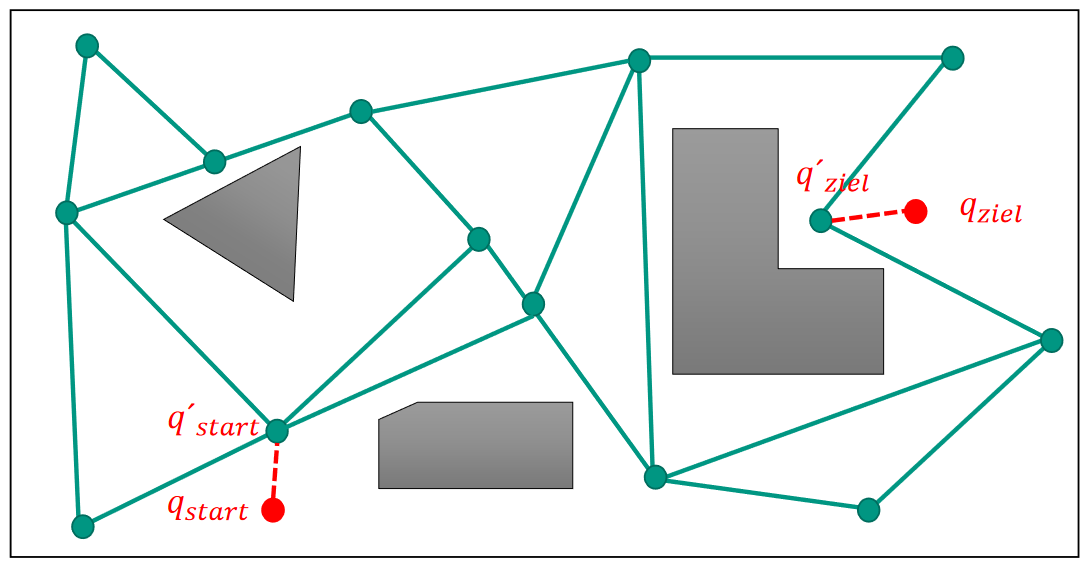
\includegraphics[width=0.6\textwidth]{images/pfadplanung.png}
	\end{center}
\end{enumerate}

\textbf{Konstruktion des Wegenetzes} $W$ durch Voronoi-Diagramme, Sichtgraphen oder  Zellzerlegung.\\

\textbf{Voronoi-Diagramme}: 
\begin{itemize}
	\item Region des Voronoi-Diagramms ist definiert als die Menge aller Punkte, deren Abstand zum Hindernis geringer ist als zu allen anderen Hindernissen
	\item Punkte auf der Grenze zwischen zwei Regionen des Voronoi-Diagramms besitzen den gleichen Abstand zum eigenen und zum benachbarten Hindernis
	\begin{center}
		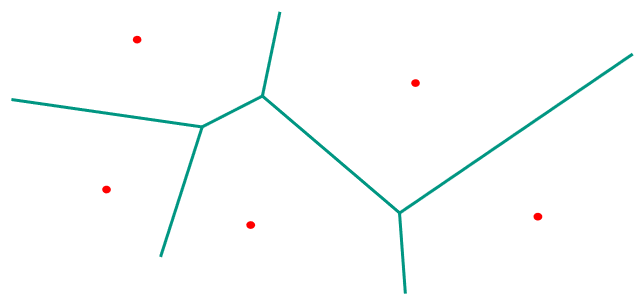
\includegraphics[width=0.4\textwidth]{images/voronoi.png}
	\end{center}
	\item \textbf{Konstruktion} mit Mittelsenkrechten, s. \textit{7/33-39}
	\item \textbf{Vorteile}: Maximaler Abstand zu Hindernissen
	\item \textbf{Nachteile}: In der Regel ist der gefunden Weg nicht der kürzeste. Bei wenigen Hindernissen werden nur wenige Wege generiert
\end{itemize}
\bigskip
\textbf{Sichtgraphen}:
\begin{itemize}
	\item Verbinde jedes Paar von Eckpunkten auf dem Rand von $C_\text{free}$ durch ein gerades Liniensegment, wenn das Segment kein Hindernis schneidet
	\begin{center}
		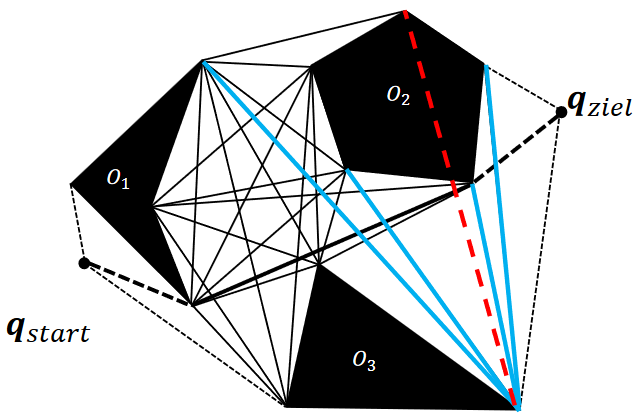
\includegraphics[width=0.4\textwidth]{images/sichtgraph.png}
	\end{center}
	\item \textbf{Vorteile}: Gefundene Weg ist optimal bei 2D-Problemen
	\item \textbf{Nachteile}: Wege sind nicht zwingend kollisionsfrei, da Hinderniskanten auch Wegsegmente sein können $\rightarrow$ \textbf{Lösung}: Erweiterung der Hindernisse
\end{itemize}
\bigskip
\textbf{Zellzerlegung}:
\begin{enumerate}
	\item Zerlege $C_\text{free}$ in Zellen, so dass ein Weg zwischen zwei Konfigurationen innerhalb einer Zelle leicht zu finden ist
	\item Stelle die Nachbarschaft in einem Graphen dar
	\item Suche den optimalen Weg von $\mathbf{q}_\text{Start}$ nach $\mathbf{q}_\text{Ziel}$ in dem Graphen
\end{enumerate}

\textbf{Exakte Zellzerlegung}:
\begin{center}
	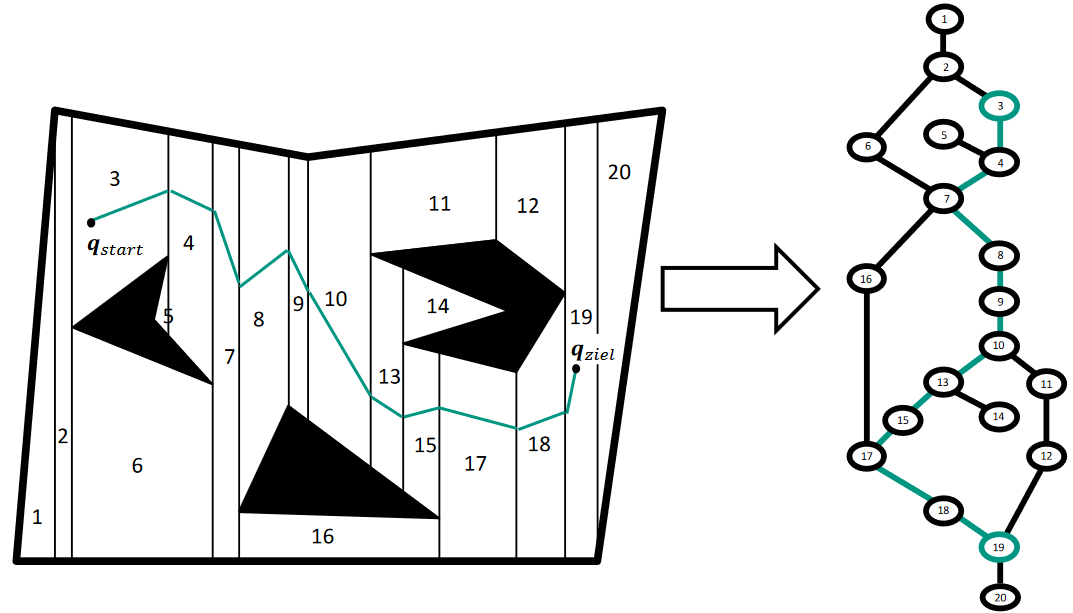
\includegraphics[width=0.7\textwidth]{images/e-zz.png}
\end{center}
\pagebreak

\textbf{Approximative Zellzerlegung}:
\begin{center}
	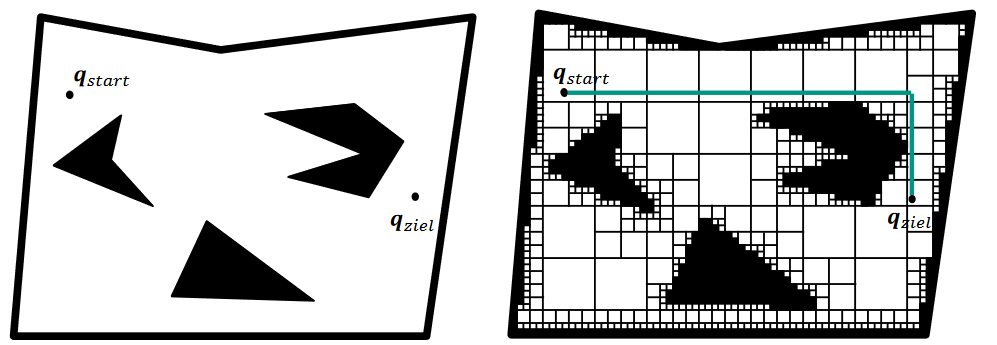
\includegraphics[width=0.7\textwidth]{images/a-zz.png}
\end{center}
\begin{itemize}
	\item \textbf{Vorteil}: Einfache Zerlegung und damit einfachere Wegsuche
	\item \textbf{Nachteil}: Freiraum kann i.A. nur annähernd beschrieben werden
\end{itemize}